\documentclass[a4paper,12pt,titlepage,oneside]{report}

\usepackage[T1]{fontenc}
\usepackage{amssymb}
\usepackage{geometry}
\geometry{
	a4paper,
	total={160mm,235mm},
	top=30mm,}
\usepackage{tabulary}
\usepackage[newcommands]{ragged2e}
\bibliographystyle{unsrt}
\renewcommand{\baselinestretch}{1.2}
\usepackage{fancyhdr}
\usepackage{algorithm2e}
\usepackage{mathptmx}
\usepackage[T1]{fontenc}
\usepackage{pslatex}
\usepackage{color}
\usepackage{cite}
\usepackage{longtable}
\usepackage{amsmath}
\usepackage{amssymb}
\usepackage{setspace}
\usepackage{lscape}
\usepackage{floatflt}
\usepackage{upgreek}
\usepackage{graphics}
\usepackage{graphicx}
\usepackage{epsfig}
\usepackage{wrapfig}
\usepackage{pbsi}
\usepackage{pdfpages}
\usepackage{bm}
\usepackage{chapterbib}
\usepackage{appendix}
\usepackage[version=3]{mhchem}
\usepackage{titlesec}
\usepackage{lipsum}
\usepackage[english]{babel}
\usepackage[autostyle]{csquotes}
\usepackage{url}
\usepackage{tabularx}
\usepackage{comment}

\newtheorem{theorem}{Theorem}
\addtolength{\belowcaptionskip}{-0.5cm}

%\usepackage{tablefootnote}
%\usepackage{footnotebackref}
%\stepcounter{secnumdepth}
%\stepcounter{tocdepth}

%%%%%%%%% Vertical Side Settings  %%%%%%%%%%%%
\setlength{\voffset}{0pt}
\setlength{\topmargin}{-0pt}
\setlength{\headheight}{12pt}
\setlength{\headsep}{25pt}
\setlength{\textheight}{660pt}
\setlength{\footskip}{30pt}

%%%%%%% Horizental Side Settings %%%%%%%%%%%%%% 
    \setlength{\hoffset}{0pt}
    \setlength{\oddsidemargin}{1.0cm}%%% Margin 
    \setlength{\textwidth}{440pt}
    \setlength{\marginparsep}{0pt}
    \setlength{\marginparwidth}{0pt}
    \setlength{\marginparpush}{0pt}
    \setlength{\headwidth}{\textwidth}
    %\setlength{\evensidemargin}{\paperwidth}
    %\addtolength{\evensidemargin}{-\textwidth}
    %\addtolength{\evensidemargin}{-4.5cm}
    %\addtolength{\evensidemargin}{-\oddsidemargin}
    
 \makeatletter
   \def\cleardoublepage{\clearpage\if@twoside \ifodd\c@page\else%
   \hbox{}%
   \thispagestyle{empty}
   \newpage%
   \if@twocolumn\hbox{}\newpage\fi\fi\fi}
 \makeatother
 \renewcommand{\topfraction}{0.95}
 \renewcommand{\textfraction}{0.05}
 \renewcommand{\floatpagefraction}{0.85}  
 
 \makeatletter
  \renewcommand{\paragraph}{\@startsection{paragraph}{4}{0ex}
   {-3.25ex plus -1ex minus -0.2ex}
   {1.5ex plus 0.2ex}
   {\normalfont\normalsize\bfseries}}
 \makeatother

%\titleformat{\chapter}[display]{\normalfont\rmfamily\huge\bfseries}
% {\chaptertitlename\ \thechapter}{20pt}{\Large}
%\titleformat{\section}
%  {\normalfont\sffamily\Large\bfseries\color{cyan}}
%  {\thesection}{1em}{}

%\def\paragraph{\@startsection
%     {paragraph}{4}{\z@}{3.25ex plus 1ex minus .2ex}{-1em}{\normalsize\bf}}
%\def\subparagraph{\@startsection
%     {subparagraph}{4}{\parindent}{3.25ex plus 1ex minus
%    .2ex}{-1em}{\normalsize\bf}}
%\renewcommand{\rmdefault}{phv} % Arial
%\renewcommand{\sfdefault}{phv} % Arial




%%%%%%%%%%%%%%%%%%%%%%%%%%%Title Page %%%%%%%%%%%%%%%%%%%%%%%%%%%%%%

\pagenumbering{roman}
\thispagestyle{empty}          %%to skip numbering on page(s)
\begin{document}
%\begin{comment}
\begin{center}
	\textbf{{\textsf{\\ SENSOR NETWORK AND VISUALIZATION FOR AIR POLLUTION MONITORING}}}
	\\~
	\\~
	\textsf{by}
	\\~
	\\~
	\textbf{\textsf{Ashlin Saju}}
	\\~
	\textsf{B.Tech, Mahatma Gandhi University, Kerala, India, 2016}
	\\~
	\\~
	\\~
	\\~
	\\~
	\\~
	\\~
	\\~
	\\~
	\\~
	\\~
	\textsf{THESIS SUBMITTED IN PARTIAL FULFILLMENT OF}\\
	\textsf{THE REQUIREMENTS OF THE DEGREE OF}\\
	\textsf{MASTER OF SCIENCE}\\
	\textsf{IN}\\
	\textsf{COMPUTER SCIENCE}
	\\~
	\\~
	\\~
	\\~
	\\~
	\\~
	\\~
	\\~
	\\~
	\\~
	\\
	\textsf{UNIVERSITY OF NORTHERN BRITISH COLUMBIA}
	\\~
	\textsf{September 2019}
	\\~
	\\~
	\textcopyright \textsf{ Ashlin Saju, 2019}

\end{center}
%%%%%%%%%%%%%%%%%%%%%%%%%%%%%%%%%%%%%%%%%%%%%%%%%%%%%%%%%%%%%%%%%%%%%


%%%%%%%%%%%%%%%%%%%%%%%%%%% Abstract  %%%%%%%%%%%%%%%%%%%%%%%%%
\doublespacing
\normalsize

\newpage
\addcontentsline{toc}{section}{Abstract}

\subsection*{Abstract}

Among the risk factors with serious health issues, air pollution ranks the highest annually. Air pollution is considered as the main cause for the majority of deaths and suffering from chronic diseases. To address this issue, we believe, active participation from the public on collecting and interpreting data, educating to change the behavior of individuals and industries, and helping to control and manage pollution sources effectively is crucial. Fortunately, this goal appears to be achievable due to the recent revolution of electronic and computing technologies. It is possible that small, portable, and off-the-shelf pollution sensors along with low power processors and wireless communication modules can be bought at low-cost. Also, to make the data available to different users we need to build a system specific software which focuses on different level of users. The need for user-specific software for general purposes are consistently increasing. The two focused tasks are first is a  system framework on how to build a low-cost portable pollution monitoring system and next is building user specific software from scratch that will focuses on different user groups.
Contributing to achieving this task is the objective of this work. We propose a portable pollution monitoring system framework using low cost off the shelf pollution sensors and demonstrate its feasibility with the software that we built in our lab.


%%%%%%%%%%%%%%%%%%%%%%%%%%% Table of Content %%%%%%%%%%%%%%%%%%%%%%%


\newpage
\addcontentsline{toc}{section}{Table of Contents} % Add to the content
\tableofcontents
%%%%%%%%%%%%%%%%%%%%%%%%%%% List of Tables %%%%%%%%%%%%%%%%%%%%%%%%%

\newpage
\addcontentsline{toc}{section}{List of Tables}   % Add to the content
\listoftables
%%%%%%%%%%%%%%%%%%%%%%%%%%% List of Figures %%%%%%%%%%%%%%%%%%%%%%%

\newpage
\addcontentsline{toc}{section}{List of Figures}   % Add to the content
\listoffigures

%%%%%%%%%%%%%%%%%%%%%%%%%%% Acknowledgement %%%%%%%%%%%%%%%%%%%%%%%%
\onehalfspacing
\newpage
\addcontentsline{toc}{section}{Acknowledgement}  % Add to the content
\section*{Acknowledgement}
%\bsifamily
%\begin{comment}

{\large
\emph{I would like to express my deep sense of gratitude to my worthy supervisor Dr. Alex Aravind for allowing me to carry out my work under his invaluable guidance. His interest in scientific problems and moral inspiration have made current work possible. I am extremely indebted to the Chairperson, Department of Computer Science, Northern University of British Columbia, Prince George, for providing all the necessary facilities to complete this work. Also, a special thanks is extended to Dr. Stephen Rader and Dr. George Jones for offering their valuable assistance as my committee members.}

\emph{I am also indebted to my labmates Apratim, Ashlin, Conan, Brae, Davis, Suresh, Shanthini, Darshik, Rahim, Ketan, Arthi, Raja and Rodrigo for their support, discussion, encouragement, and pleasant company. Special thanks to the teaching and nonteaching staff members, UNBC, for their help in all possible ways.}
\par
\emph{It is a pleasure to acknowledge the good company of fellow researchers and my friends Hardev, Gurjeet, Ashish, Ramneesh, Johny, Priyanka, Amit, Navjot, Bashet, Dorob and many others.}

\emph{Finally, I want to express my deepest gratitude to my family for their love, support and encouragement, without which this work would not have taken this shape.}

\vspace{1.0cm}
%\begin{tabular}{p{4.5in}r}
\emph{Prince George, BC}

\emph{September~~~~, 2019\hfill\textbf(Ashlin Saju)}
%\end{comment}
%\end{tabular}

%%%%%%%%%%%%%%%%%%%%%%%%%%%% Dedication Page %%%%%%%%%%%%%%%%%%%%%%%%%%%%%%


\setstretch{0.7}
\newpage
\thispagestyle{empty}
\addcontentsline{toc}{section}{Dedication}
\begin{tabular}{p{4in}cr}
	 &  &                                                                          \\&&\\&&\\&&\\&&\\&&\\&&\\&&\\&&\\&&\\&&\\&&\\&&\\&&\\
	\emph{\textbf{\large{~~~~~~~~~~~~~~~~~~~~~~~~~~~~~~~~~~~~~~~~~~~~Dedicated}}}  \\&&\\ \emph{\textbf{\large{~~~~~~~~~~~~~~~~~~~~~~~~~~~~~~~~~~~~~~~~~~~~~~~~~~~to}}}\\&&\\
	\emph{\textbf{\large{~~~~~~~~~~~~~~~~~~~~~~~~~~~~~~~~~~~~~~~~~~~~My Parents}}} \\
\end{tabular}

%%%%%%%%%%%%%%%%%%%%%%%%%%%%%%%%%%%%%%%%%%%%%%%%%%%%%%%%%%%%%%%%%%%%%%%%%
%\end{comment}


%%%%%%%%%%%%%%%%%%%%%%%%%% CHAPTERS %%%%%%%%%%%%%%%%%%%%%%%%%%%%%%%%%%%%

\doublespacing
\normalsize

\newpage

\fancyhead{} % clear all header fields
\fancyfoot{} % clear all footer fields
\pagestyle{fancy}
\fancyhfoffset[L]{0 cm}
\rhead{\text{\thepage }{}}
\fancyfoot[C]{Footer} %ashlinchange
\fancyfoot[C]{}% \fancyfoot[R]{\thepage} %ashlinchanges
\renewcommand{\footrulewidth}{0.4pt}% Default \footrulewidth is 0pt ashlinchanges
\lhead{\textbf{\chaptername\hspace{0.1cm} \thechapter{}}}

\titleformat{\subsection}
{\normalfont\large\bfseries}   % The style of the section title
{}                             % a prefix
{0pt}                          % How much space exists between the prefix and the title
{\thesubsection\quad}

\titleformat{\section}
{\normalfont\Large\bfseries}   % The style of the section title
{}                             % a prefix
{0 pt}                         % How much space exists between the prefix and the title
{\thesection\quad}
\doublespacing

\chapter{Introduction}
\pagenumbering{arabic}
\setcounter{page}{1}


TRYING T SEE IF GIT WORKS

Earth, Our home planet, is the only place in the known universe affirmed to host life. The life on earth is characterized by three components, Air, Land, and Water. Each element has its own special properties and required in its proper proportions to maintain the healthy life of all living beings \cite{environment}. The quality of life is relied upon the quality of environment. The Ecosystem with its creatures and vegetation ought to be sound with clean assets, clean water and air.  However, the improper ways of industrial development and  other manmade activities creates a disturbance in the natural environment. This process of making land, water, air or other parts of the environment unsuitable and unsafe for living is called pollution. 
\par
Pollution is a universal phenomenon that degrades the land, air, water bodies, and structures by the introduction of contaminant into the natural environment. This changes the quality of atmosphere and are trans boundary, as they travel thousands of miles  \cite{environment}. Organic pollutants which contains organic compounds are non-biodegradable and resist degradation by microorganisms; therefore they remain in the ecosystems for quite a while. 
The environmental scientists these days mainly face the problems related to the global warming and climate change. Out of different types of pollution, Air pollution plays a major role for global warming.
\par
 Air contamination alludes to release of pollutants into the environment that is unfavorable to human wellbeing and the planet in general. Air pollution is stated as a complex mixture of gases and particles whose sources and composition vary over space and time \cite{HealthEffectsInstitute2017}. The boom in the development of industries and technology have created an alarming situation tha is, degrading the quality of air. Contamination of air is a matter of serious concern and society is less aware of the impact that it causes to human health as well as to the surrounding. The World Health Organization (WHO) reported that 9 out of 10 people breath polluted air which estimates a death rate of around 7 million every year \cite{who} \cite{WHO2010}. This has made many motivated individuals like researchers and communities to work towards in creating awareness among the people. There are already different studies going on air pollution due to its increasing effects on the environment day by day. I choose to work on sensor network for air pollution since its an application level problem and also because of my background in electronics. In the next section I will discuss the background to introduce my research work.


\section{Air Pollutants and Measurement Metrics}


There are various pollutants that contribute to the contamination of the environment. These pollutants differs from region to region depending on the activities. In the industrial area which manufactures products from raw material such as production of iron from its ore or production of gasoline from crude oil releases inorganic carbon compounds into the atmosphere \cite{Vallero2014}. Urban areas are the major sources of the particulate matter, Ozone and carbon compounds from the burning of fuels in the vehicle.
Based on the severity of health impact and the kind of activities, the the National Ambient Air Quality Standards (NAAQS) has set six common criteria pollutants that harm health, environment or even property damage. The NAAQS was established by the United States Environmental Protection Agency (EPA) under the Clean Air Act which specifies the pollutants that are harmful for the public health and environment \cite{USEPA} \cite{NAAQS}. The criteria pollutants are particulate matters ($PM$), ozone ($O_3$),  nitrogen dioxide ($NO_2$), carbon monoxide ($CO$), sulphurdioxide ($SO_2$), lead ($Pb$).

Different countries measures different set of pollutants, for example, India measures 8 major pollutants such as particulate matters ($PM$), ozone ($O_3$),  nitrogen dioxide ($NO_2$), carbon monoxide ($CO$), sulphurdioxide ($SO_2$), ammonia ($NH_3$), and benzene ($C_6H_6$) (in some places lead ($Pb$) instead). Most other countries measures a subset of these criteria pollutant for example, Canada measures $PM, O_3, NO_2, SO_2$ and $CO$ \cite{Chen2013}. Particulate matters are measured at two levels; 2.5 micron size particles ($PM_{2.5}$) and 10 micron size ($PM_{10}$), and they are measured in micro-grams per cubic meters ($\mu g/m^3$). $CO$ is measured in parts per million ($ppm$) and other gases are measured in parts per billion ($ppb$). These individual measurements make less sense to the common public and therefore are not very helpful in understanding the cumulative impact of the air quality. Taking this into account the government agencies of each country developed their own indices corresponding to the National Ambient Air Quality Standards (NAAQS)  for representing the quality of air. The different indices are Air Quality Health Index, Air Quality Index, Air Pollution Index, Pollution Standard Index, Comprehensive Air Quality Index, Daily Air Quality Index, Common Air Quality index are few used in different countries.
Out of all these indexes the most common are AQI and AQHI which are proposed and used by different countries \cite{Chen2013}.

India, USA, UK, and many other countries use AQI and Canada, Hong kong uses AQHI. These metrics are designed  by carefully examining those pollutants which are harmful to human health and environment.
AQI is a piecewise linear function of the pollutant concentration \cite{Soni2016} and is measured using the following formula.

\begin{equation}
AQI = Max \{I_i|i = 1, ..., 8\}
\end{equation}
where $I_i$ is an air quality subindex corresponding each pollutant and it is computed as 
\begin{equation}
I_i = \lceil(\frac{I_{high} - I_{low}}{C_{high} - C_{low}})\rceil \times (C - C_{low}) + I_{low}
\end{equation}
where $C$ is concentration of the $i^{th}$ pollutant. $C_{low}$ and $C_{high}$ are lower and upper concentration breakpoints of $C$ respectively.
$I_{low}$ and $I_{high}$, respectively, are index breakpoints corresponds to $C_{low}$ and $C_{high}$.  The value of AQI varies from 0 to 400+ as shown in the figure \ref{aqi} and each colour code shows the quality of air in the atmosphere.


\begin{figure}[h]
    \begin{center}
    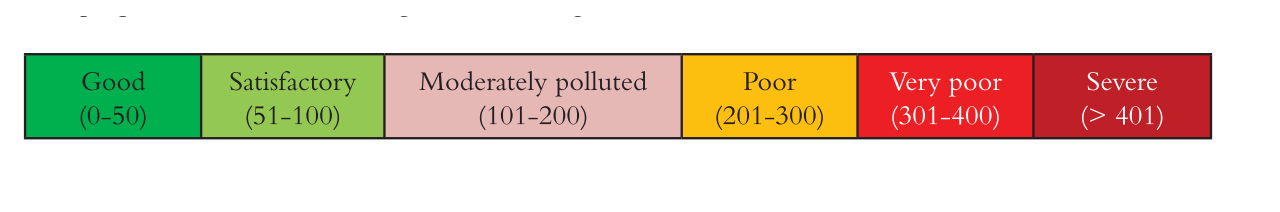
\includegraphics[scale=0.58]{./images/figure13.png}
    \end{center}
   
    \caption{Air Quality Index (AQI) \cite{AirQualityIndex}}
    
    \label{aqi}
\end{figure}


In Canada, the Environmental agency developed AQHI to make the common public aware about the air that surrounds them. It was based on five major pollutants $PM_{2.5}$, $O_3$, $NO_2$, $SO_2,$ and $CO$ initially and later the last two pollutants were dropped from the calculation as they were identified to  contribute very less in predicting health effects. AQHI computed using the following formula.


\begin{equation}
AQHI = \lceil (\frac{1000}{10.4}) \times [e^A-1]+[e^B-1]+[e^C-1] \rceil
\end{equation}

where $ A = 0.000537 \times$ concentration of  $O_3$, $B = 0.000871 \times$ concentration  of $NO_2$ and  $C = 0.000487 \times$ concentration of $PM_{2.5}$.
The value of AQHI varies from 1 to 10+ as shown in figure \ref{aqhi}


\begin{figure}[h]
    \begin{center}
    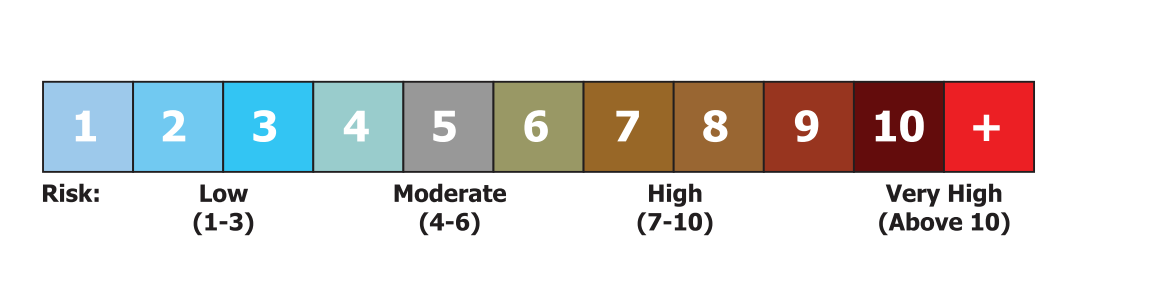
\includegraphics[scale=0.58]{./images/figure12.png}
    \end{center}
   
    \caption{Air Quality Health Index (AQHI) \cite{healthcanada}}
    
    \label{aqhi}
\end{figure}

Now the question is which is a better measure, AQI or AQHI? Health index was created with a different objective which is to provide a combined effects of pollutants to the human health. AQI is based on a single pollutant and hence it is hard to see its direct relationship with health compared to AQHI \cite{Chen2013}. On the other hand AQHI is based on the  the exposure-response relationship between the major air pollutant mix and human health \cite{Chen2013}, which gives more close relation to the mixture of air pollutant than AQI. It is to be noted that both the indices failed to project the health outcomes associated with the exposure to the polluted environment.



\section{Impact of Air Pollution}

Air pollution has significantly increased after the industrialization and urbanization have taken place. The burning of fossil fuels, exhaust from factories and industries, and mining operations are the major contributors to air pollution. The exposure to air pollutants causes premature deaths, cardiovascular disease, stroke, and other respiratory diseases. The state of global air 2017 has discussed the effects of long-term exposure to harmful air pollutants such as particulate matter which contributes to over 4 million premature deaths and is estimated to
double by 2050 if the issue remains unattended \cite{HealthEffectsInstitute2017}. Among the risk factors with the serious health issues, air pollution ranks the highest annually accounting for majority of deaths. The major impacts of air pollution are premature deaths, cardiovascular disease, stroke and other respiratory diseases.
Particles with a diameter of less than 10 microns ($PM10$), and less than 2.5 microns ($PM2.5$) causes the greatest threat to health, as they are capable of penetrating to lungs which leads to cardiovascular and chronic obstructive pulmonary diseases (COPD). \cite{who} \cite{Tian2016}. Exposure to carbon monoxide ($CO$) which is a colorless and odorless gas is absorbed into bloodstream from lungs and reduces the ability to transfer oxygen which inturn affects the functionality of organs such as brain and heart \cite{Sierra-vargas2012} \cite{Golbabaei2012}. Respiratory issues such as decrease in responsiveness of airways, inflammation in airways, lung infectivity occurs due to exposure of high concentration of ozone ($O3$) \cite{Lippmann1989}. Another pollutant is nitrogen dioxide ($NO2$) which causes such as wheezing, coughing, bronchitis and flu. The exposure of mixed air pollutants leads to diverse health effects like birth defects, development delays in children, skin irritation or even cancer \cite{MarilenaKampa2007}.

\section{Background}

The quality of the air has declined since the industrialization has taken place in the mid 19th century. Ever since then it has affected not just the environment but also the human health. There was a development of heavy industries across Europe to North America which used coal as their major source of energy that contributed to black smoke pollution \cite{Heidorn1978} \cite{Timothy}. Coal was not just used in industries but also in houses for heating in winter which made the pollution even worse \cite{Al2016}. These emissions resulted in serious health impacts on residents in urban areas that increased the mortality rate during this period. One such important event in the history of pollution is the great smog of London which killed as many as 12,000 people to death mostly infants. This was caused due to the combination of cold weather with smoke and lasted for several days \cite{londonfog}. There were a string of similar events reported in New York, England, Britain around the same time. All these incidents led to the development of Environmental Protection Agency (EPA) who enforced the need for installing the monitoring stations. The government along with these environmental agencies established acts like clean air act, motor vehicle air pollution act, air pollution control acts for a better quality of air\cite{airpollutionact}. Apart from that they took initiative to monitor the air pollution by installing systems which could measure the concentration of pollutants and could give warnings to public as well as industries regarding the  polluted atmosphere.


\subsection{Existing Environmental Monitoring station}

The government and the Environmental agencies are taking an effort for installing monitoring stations for improving the air quality. The EPA monitors the criteria pollutants along with any special pollutant dominant in that particular area. These monitoring stations are fixed in a particular location and are operated by environmental agencies. These stations are equipped with instruments not just criteria pollutants but also analyzes other parameters like wind speed, humidity, precipitation. These analytical instruments works by the principle of sampling of the air collected from the atmosphere.
There are two main methods for pollutant sampling: 1) passive sampling, and 2) active sampling \cite{Balakrishnan2015} \cite{activepassive}. These sampling techniques are considered as one of the most significant development for air quality measurement. These approaches are used widely for monitoring purpose. In passive sampling the pollutants are collected by physical process such as diffusion through a static air layer or membrane. These pollutants in the air is diffused to adsorb on the sampling media due to difference in the chemical composition of pollutants. The analysis of the pollutant on the sampling media will give the time-averaged contaminant concentration \cite{Environment2009}. on the other hand, in active sampling there is a use of an air sampling pump which actively pulls the air through a collection device like filter  and weighted concentration is calculated. However these static instruments have a major drawback of temporal resolution as they are large in size and needs high maintenance. These instruments are expensive and are financially impractical to expand more station. The table \ref{table:cost} gives the average estimated cost for purchasing air quality monitoring equipment produced by US Environment protection agency. 

\begin{table}[h]
  
  
    \begin{tabularx}{\columnwidth}{X|X}
        \hline
        Pollutant/Parameter           & Estimated cost    \\
        \hline
    
      $NOx$   & 10,4440  \\ 
      $SO2$   & 35,000  \\ 
      $COx$   & 28,000  \\ 
      $Ox$   & 6,600  \\ 
      $PM$   & 37,700  \\ 
     
      FTIR Analyzer   & 100,000 \\ \hline
     
        
      
  \end{tabularx}
  *FTIR: Fourier Transform Infrared spectroscopy measures multiple gases 
    \caption{Estimated cost of Reference Instruments(USD) \cite{Mussatti2000}}
    \label{table:cost}
  \end{table}


As a result of high cost there can only be few monitoring stations installed for a particular area. Thus we can claim that spatial resolution is limited by these conventional monitoring equipments. This made the researchers and scientists to work more on portable sensor networks to understand more on air pollution.



\subsection{Sensor Network for Air Quality Monitoring}

There is an emerging trend of using air sensors to understand the quality of air because of its low cost, small size and low power consumption \cite{Sun2016}. These sensors are way cheaper than reference station and can be replaced easily in case of any damage. The advancement in the micro-electro-mechanical (MEMS) system made it possible to integrate all the functions into a single electronic circuit which makes it more compact. These sensors do not need any deployment cost, infrastructure cost or any frequent maintenance which makes the overall expense even less. There is a huge amount of other application which could be achievable with sensor such as military monitoring purpose, surveillance and tracking, traffic density calculation and road condition and environmental application \cite{Kadri2013}. The sensor unit can be accommodated with an automobile, building tops or even could be worn in order to track. This enables high spatial resolution without establishing huge reference station \cite{Nodes2015}. Sensors measuring different compounds are integrated together to make a sensor node system. There are many research work done with the available sensors in the market. 





\section{Motivation}

One of the important components in solving this issue is to increase the awareness among public about the current situation and its impact so that they can act on it. The conventional method of monitoring the air quality with the help of a few heavyweight expensive stationary monitoring systems typically installed by the state may not be effective enough for this task. To achieve the goal effectively and without further delay, pollution monitoring must become part of daily activity for everyone. For that the devices to monitor pollution must be small, portable, inexpensive, and part of a global system. With the technological advancement of low cost computing, communication, and sensing devices, and the revolution and the importance of open source software \cite{Anthes2016}, we believe it is possible to build pervasive air pollution monitoring system with commodity hardware and open source software. Now the question is how to design such pollution monitoring devices faster and make them accessible to as many as possible. 
\\
Achieving the above stated goal requires a suitable system framework that can help to accelerate the process of the design and implementation of a air pollution monitoring system using the off-the-shelf commodity hardware and open source software. There are some recent attempts in this direction, but none is comprehensive and simple enough to follow and build a air pollution monitoring system with a little or moderate effort. This thesis is an attempt to fill that gap by first proposing a simple and comprehensive framework and then demonstrating its feasibility and use by creating our own pollution monitoring system that is operational in our lab. We have also added a step of calibration by implementing a web-based tool to find out the quality of data obtained from the system. Our contribution is a step towards inspiring and motivating not only the public to use the device, but also many amateur electronic hobbyists to buy the hardware locally and download the associated software to build their own pollution monitoring device.


\section{Research Problem}
The aim is to design and develop an air pollution monitoring system using off the shelf
hardware and open source software and analyze the quality of data obtained through calibration with the following objectives in mind.
\begin{enumerate}
    \item To develop a calibration tool which could give how accurate the sensor data is when compared with referance data.
    
    \item To educate the common people on adverse effect of air pollution by showing how polluted
    the vicinity is.
    
    \item To influence the behaviour of people by representing the concentration of pollutant as well
    as AQHI (Air Quality Health Index) which provides the seriousness that pollutants cause
    to health.
    
    \item To give an idea of how to integrate all the hardware components to a processor and also
    make an independent software, which can be accessed anywhere in the world.
    
    \item To encourage and help citizen science to solve the issue of air pollution and give more
    understanding to the impact it cause to human health and environment.

\end{enumerate}


\section{Thesis Contribution}


\section{Research Question}
 
 Some important research questions to be addressed related to the issue of air quality are: 

 \begin{enumerate}
  \item What kind pollutants affect the human health most? How to measure them?
   
  \item  As the pollution is in the atmosphere, should it not be measured everywhere all the time? If so, what kind of infrastructure is needed to facilitate such a ubiquitous measurement?
  
 \item What all factors should be considered while selecting sensors for measurement of pollutants?
 
 \begin{enumerate}
 \item Accuracy of the data collected from the sensors.
 \item The cost of the sensors.
 \item The size of the sensors.
 \item Integration with the processor.
 \end{enumerate}

 \item Which processor to be used for processing the data collected from sensors?
 
 \begin{enumerate}
 \item The ability to process analog signals collected from the sensor.
 \item Opens source platform.
 \item Ability to use in real time application.
 \item Able to connect with the Wi-Fi module easily.
 \end{enumerate}

 \item How should the hardware component i.e the sensors and the processor, should be packaged?
 
 \begin{enumerate}
\item As compact as possible.
\item The value of the sensors should not be affected.  
 \end{enumerate}
 
 
   \item What is the difference between different metrics which is used to show       	the effect of pollution?
   \begin{enumerate}
   \item Understanding why different indexes are used for pollution monitoring.
   \item To identify which all indexes should be displayed in the software.
   \item Out of all the indexes which one is the most relevant to public and why?
  
   \end{enumerate}
  
 \item How can the seriousness of pollution be made aware?
 \begin{enumerate}
 \item What all graphs or charts to be used?
 \item How to make a impressive software tool for demonstration?
 \end{enumerate}
 
 \item How can the representation of Air quality metrics be done?
\begin{enumerate}
\item Should there be any categorization within the society for data visualization?
\item If so, what all data should be shown for each section?
\item How to demonstrate a simple view of complex effectively?
\end{enumerate}
 
 

 
 \end{enumerate}
 
\section{Research Challenges}


The major challenges expected on creating a complete system are:

\begin{enumerate}


\item The integration of different sensors with the processor.
\par
As each sensors are having its own properties, there can be a issue when connecting all of them together in a single platform. Most of the sensors used for measurement are heat sensor and needs to be powered atleast 12 hours before operating. There is a particular operating temperature range for each sensors connected. As each of the sensor needs different environment for working, all the factors should be incorporated for a complete working environment.

\item Integration of communication module which is  WiFi with processor as this module alone requires a different voltage level to drive.
\par
The data transferring module used here is a WiFi module which needs a separate voltage level of 3.3 Volt when compared to the sensors which are driven with a voltage of 5 Volt each. On giving any voltage more than 3, will burn the entire module and hence it needs a separate voltage line to be given. 

\item Calibration of each sensors based on the data sheet.
\par
As I am selecting commodity sensors which says that it is already calibrated but usually it should be done for each environment. The data collected changes for each environment and this should be taken care of. This can be a tough task as for each of the sensors it changes based on the slope of internal resistance and the internal voltage values given in data sheet. 
\item Packaging of hardware component.
\par
To make the whole system portable it should be packed carefully. For certain sensor like dust sensor, it should be exposed to the environment so as to get the value of particulate matter. This packing should be done in such a way that the it does not hinder with the observed value.

\item Transferring the data to a platform or a database using the WiFi module.

\item Checking whether the collected data is accurate.


\end{enumerate}

\section{Structure of the Thesis}    %%%% Input file with Chapter1.tex
\chapter{Literature Survey}

Development of Wireless Sensor Network (WSN) is considered as one of the matured innovation in the field of electronics. The miniaturization of the components has allowed the user to explore applications in various fields such as health care, military applications, traffic control, monitoring, and data collection \cite{Khedo2017} \cite{Liu2017}. Out of all the applications, urban air quality monitoring has gained a lot of attention as it is one of the major issues faced by society today. While reviewing the related work, we found out that there are various methods used for understanding pollution. This could be classified into four based on literature as follows \cite{Yi2015} \cite{Pavani2017}.




%There are different approaches for measuring air pollution and this chapter gives an overview of the research work done for understanding this based on the medium for measurement. The popular mediums used for the measurement can be classified as below
 
\begin{enumerate}

    \item Vehicle-based sensor network
    \item Wearable sensor network
    \item Community sensor network
    \item Static sensor network

 \end{enumerate} 

 Further we will be highlighting the important research done in each of the above four categories and will be classifying to which category our work falls.

\section{Vehicle based sensor network (VSN)}

In recent times, the number of private vehicles on the road has increased in proportion to the increasing population around the globe \cite{Downs2004}. Even though the increase in the number of automobiles is one of the major factors that is contributing to the increase in pollution, certain researchers took this as a medium for measuring air pollution data. In this category of work, the vehicles (like buses or cars) are installed with a portable, low-cost sensor to obtain spatially resolved data. 
\par
%Portable and low-cost sensors are installed and attached to a vehicle like buses or cars in order to achieve a spatially resolved data. There have been an increasing number of mobile vehicles in urban areas. This was taken as a medium for obtaining air pollution data from the environment in cities. 
 One of the best ways to study the quality of air is by collecting fine-grained data also called \lq{micro-climate monitoring}\rq. However, with the existing monitoring system being bulky and expensive it is impossible to obtain spatially resolved data. To solve this issue, in 2009 a group of researchers used mobility as a method and proposed a vehicular wireless sensor network \cite{Hu2009} that measures the changes in concentration of a single pollutant measurement (Carbon Dioxide in this case) by mounting the sensor node onto a vehicle. The system is equipped with a Carbon Dioxide ($CO_2$) sensor, a Global System for Mobile (GSM) module, a GPS receiver, and a ZigBee module to create an intra-vehicular network. The collected data is transferred through GSM short messages to the server and is displayed on Google Maps for results. The architecture of the VSN is shown in the figure\ref{vsn}. 

 \begin{figure}[h!]
  \begin{center}
  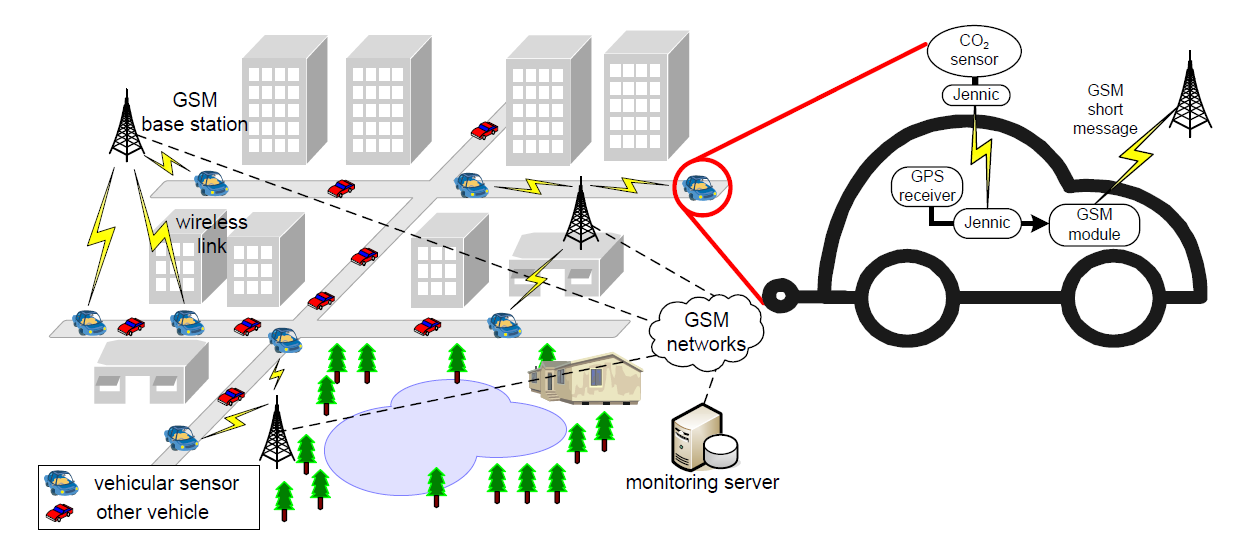
\includegraphics[scale=0.65]{./images/figure40.png}
  \end{center}
 
  \caption{Architecture of Vehicular based sensor network \cite{Hu2009}}
  
  \label{vsn}
\end{figure}
 
 This work faced two network-related drawbacks. Firstly there was a duplication of air pollution data as the number of vehicles in a given area changed dramatically from time to time and secondly, to reduce the data transfer in an area with many sensor nodes at the same time by exploiting opportunistic communication. These two problems were later addressed in 2011 \cite{Hu2011} by designing two message-efficient algorithms. The first algorithm works by dividing the sensing field into a fixed number of grids and each grid was allocated with a particular reporting rate which is called dynamic reporting rate to reduce communication overhead. The second algorithm allows the sensing nodes to communicate with each other and find out their reporting rate and opportunistically transfers the collected data. %The main area of the work revolved around data collection, optimization of the collected data, and concentrating only on one pollutant. The other issues like the quality and accuracy of the collected data, management and operations of wireless sensor networks were not given priority.



 %They also created a simulation model to verify the performance of the algorithm. The above two research work mainly focused on data collection, optimization of the collected data, and only revolved around one pollutant. The problems like calibration of sensors, visualization of data, checking the accuracy of the collected data, and management of the VSN was not taken care of.
\par

 Volgyesi et al. \cite{Volgyesi2008} proposed the Mobile Air Quality Monitoring Network (MAQUMON) that measured three pollutants, Ozone ($O_3$), Carbon Monoxide ($CO$), and Nitrogen Dioxide ($NO_2$). The air pollution system is mounted on a car and is powered by a Li-ion battery whose battery life is limited to a few hours. It is equipped with a GPS module for determining the location and the collected data is transferred to a laptop through a Bluetooth module. When the system is in coverage of a Wi-Fi network the collected data is transferred to a web server and visualized in sensor map web application in the form of contour maps. %However, the inability of representing instantaneous data is one of the main concerns with this system and also have failed to show the accuracy of collected data to the local system.


\par


The data collection that involves more frequent and spatially dense pollutant measurement is called a fine-grained approach. In \cite{Devarakonda2013}, the vehicular-based approach of measuring
fine-grained air quality in real-time was demonstrated. To increase the spatial density the study proposed two data collection models one for public transportation infrastructure and the other for a personal sensing device. A Mobile Sensing Box (MSB) was installed in public transit buses which contained the microcontroller (Arduino), sensors for measuring Particulate Matter ($PM$), Carbon Monoxide ($CO$), a GPS module and a cellular modem. The module was powered through the bus batteries and the collected data were transferred to a server and visualized using Google Fusion tables interfaces. In the second framing, a Personal Sensing Device (PSD) that included an air quality sensor was installed in cars and connected via Bluetooth to a smartphone. This gave the user information about the air quality while driving through a specific area.
The data obtained from both the framing models were compared using linear regression and the results showed a positive linear relationship between the data sets. Even though there was a high correlation seen between the two sets of data there was no comparison with the local reference data to understand the accuracy of the system.

\par

A similar technique of data collection like in \cite{Devarakonda2013} can be seen in wireless sensor deployment \cite{Saha2017} that proposed the idea of placing the sensor nodes in public transport buses to obtain real-time data of pollutants. The system here is divided into sensor node and sink node in which the former collects the data from the environment and the latter aggregates the data from the sensor node and transmits to a server via a long-range radio band. These sink nodes are either installed in a T-junctions or an X-junction of the city where most of the buses cross. The data is transferred at a regular interval of time and can be analyzed instantly. However, the paper did not discuss the collection of data and failed to provide the quality of collected data.



A research group from Japan, Shirai et.al \cite{Shirai2016} proposed an effective method to acquire air quality data in an urban areas in which the air pollution system has a sensing unit kept on a public vehicle like a garbage truck and garbage patrol vehicle which moves in and around the city. The main focus is on pollutants like Particulate Matter ($PM$), Carbon Monoxide ($CO$) and Sulphur Dioxide ($SO_2$), and is also aided with GPS module. To remotely monitor the sensing conditions and to check for maintenance, a control center tool has also been developed. It consists of a map that tracks the route of the vehicles and the sensor data acquired by each vehicle. A monitor was developed along with the system to send the users the collected data. It estimates the amount of pollution inhaled by the user like one in \cite{Devarakonda2013} which by acquiring the user's location from the mobile application and mapping it to the location-sensors value which has been already computed. It also considers the respiratory volume of the user to estimate the pollution inhalation.

Another mode of transportation that was taken for understanding the air quality was the public bicycle system. The bicycle borne sensor \cite{Xiang2016,Liu2015a} deploys a system equipped with an exhaust gas sensor, Particulate Matter ($PM$) sensor, GPS module, and a microprocessor. The system collects data along with the location from the GPS module and is stored in a micro storage chip. The system is powered with the help of Lithium polymer batteries. When the subscriber returns the bicycle to the dock station the data is transferred to the data center via the Bluetooth module and is then visualized using the 'Baidu' heat map.

In \cite{Zhi2017}, Unmanned Aerial Vehicle (UAV) is used as a medium to understand air quality.  In contrast to the work done in \cite{Hu2009,Hu2011,Volgyesi2008,Devarakonda2013,Shirai2016,Xiang2016,Liu2015a,Saha2017} this work focused on six different pollutants that contribute to Air Quality Index by mounting the sensor board on the flight. The flights are carried out in 30 days with 20 minutes of monitoring. Along with the sensor board, a smartphone is attached that collects data from the air sensor by establishing a Bluetooth connection. The collected data is transferred to air quality analysis software that will display the real-time monitoring value along with AQI value. 

The existing studies in this section show that collecting data using VSN supports micro-climate monitoring. The advantage of having spatially resolved data is that it helps to understand the trends of pollution in a better way. At the same time, the probability of having redundant data due to traffic congestion or duplication of data is high. Another concern is that there was no effort taken to understand the quality of data obtained. The main idea of deploying the system is to educate citizens and make them aware of the quality through the indexes. 
The efforts to calculate AQI or AQHI is not taken as a priority except in \cite{Zhi2017}. The representation of these indexes will make people aware of the air quality but most of the work in this category has failed to bridge the data gap.


\section{Wearable sensor network}


The individual effect of pollutants on health depends on the extent to which a person is exposed to the polluted environment. The understanding of the health effects could be achieved by observing the exposure-response relationship \cite{Dons2017} this will give an idea about the amount of pollutants inhaled by an individual. This could be achieved by using a wearable sensor which helps to understand the effects of individual impact when exposed to polluted air. Research was done in this section mainly focuses on improving the understanding of personal health and exposure to air pollution \cite{Hu2015}. One such development is Mypart \cite{Tian2016}  from the University of California, which is a wrist-worn particle sensor that measures particulate matter of 10 microns or less.  The design of MyPart is based on a traditional laser-based photodiode system with improvement in airflow to remove light leakage, integration of structural design and circuitry for ambient visualization, BLE transceiver for low power networking, and also a mobile application for visualization. Two main issues tackled by MyPart is accuracy and calibration of sensor which no existing consumer sensor has addressed.

Another related work is 'Eco-mini'\cite{Fletcher2015} which is a wearable stand-alone device for clinical use that measures Volatile Organic compounds (VOCs), sound level, air quality, temperature, and humidity values. This system is based on a low power microcontroller (Atmel Xmega 128k) and consists of a GPS module for position identifying and a Bluetooth module for data transfer. They modified the webserver which was developed on a simple javascript application. The next wearable work is 'citisense' \cite{Zappi2012} which is a system attached to a bag stripe which measures air pollutants like Nitrogen Dioxide ($NO_2$), Carbon Monoxide ($CO$), and Ozone  ($O_3$) along with environmental parameters such as temperature, humidity, and barometric pressure. The collected data from the sensor is processed by the microcontroller (ATMEGA1284p) and transfers the data using a Bluetooth module to a smartphone which does the data storing, analysis, and data aggregation. The collected data is then transferred to a back-end webserver from where the user can get a personalized view of their data. They also developed a citisense android application that runs on the smartphone.
 
In \cite{Kim2010}, the research group in the US developed an expressive T-shirt called 'WearAir' which indicates the measured Volatile Organic Compound (VOC) through expressive patterns. The T-shirt is designed with a metaphor of a car emitting gases with four vertical arrays of LEDs which shows different frequencies depending on the concentration of VOC gas in the surrounding. When the wearer is exposed to dense VOCs the LED will blink rapidly. 
The authors of \cite{Hu2014} developed a novel system consisting of several sensors that give real-time feedback on an individual's exposure dose. This consist of arm sensors, chest sensor or even wrist sensors which measures various pollutant concentration ($CO$ in this case) and transfers to an android or ios application via Bluetooth. They also calculate the inhaled dose of pollutants by calculating the volume of air inhaled into a person's lung per minute through an algorithm developed in \cite{Valli2013}. The inhaled dose of the pollutant was calculated and compared during various activities like jogging, bicycling, and driving.

 There are also wearable sensor projects initiated in Vancouver in association with the University of British Columbia like TZOA \cite{tzoa} that can be clipped to the clothing and measures the air quality. It mainly measures $PM$ values and display in an application. These devices decrease the gap between individual and their understanding of the polluted air. In NewYork a striking project named 'Aircasting'\cite{aircasting} provides the health and environment data using the android 'Aircasting app'. The 'Aircasting'\cite{Han2010} platform includes a palm-sized air quality monitor that measures $PM_{2.5}$, relative humidity, and temperature. The outside air is drawn through a sensing chamber and the particles are measured through the light scattering method. It also includes a LED wearable apparel named 'Air casting luminescence'\cite{Luminescence} that illuminates LEDs according to the obtained sensor measurement; varying from red for high intensity, then orange, then yellow, and finally green for low intensity. 
 
 The emergence of such wearables makes individuals be more cautious about their health and encouraged people to stay fit. At the same time, the public is not aware of these devices and does not prefer wearing T-shirts or carry a device for understanding the impact of pollution. Another issue to be focused on is the cost and stability of connection due to which the measured data values won't be able to visualize.



\section{Community sensor sensor}

The development of portable sensor devices has paved way for a novel paradigm for monitoring the pollution known as crowdsourcing or participatory sensing. This gives an opportunity for any citizen to collect data and transfer it to a common platform like a web interface. The collected data from the participants give a spatiotemporal view of the effect of pollution \cite{Kanhere2013}. In Sydney, a low-cost participatory system is deployed named 'Haze-watch' \cite{Sivaraman2013} for monitoring pollution in urban areas. In this, mobile sensor units were attached to vehicles, and collected data were transferred using Bluetooth to a mobile application which tags its location with date and time information. This data is then sent to a cloud-based server that stores data and applies interpolation models \cite{Liao2006} to generate Spatio-temporal estimates. Then using a web application the geo-referenced data is depicted as a contour map. 
\par
Intel has developed a prototype named 'Common Sense' \cite{Dutta2009} which is based on mobile participatory sensing \cite{Abdelzaher2007} that enables citizens to collect relevant data and involves in the decision making process. The system includes a handheld device that measures a couple of pollutants and uploads the value for visualization over the web using Bluetooth or GPRS radios. This work was further tested by deploying it on a municipal fleet of street sweepers in the city of San Francisco \cite{Aoki2008}. Another community-driven sensing developed is 'OpenSense' \cite{Aberer2010} which focuses on the utility of data by giving an idea about how the data collected from sensors needs to be consumed. They have provided two use-cases first one is smart healthcare which by giving alerts on identifying the pollution-induced diseases (like asthma, particle allergies, etc.) and next is urban planning by identifying polluted areas and identifying alternative routes. The system is deployed on mobile vehicles and stationary stations in Switzerland and the collected data is pipelined to a Global Sensor Network (GSN) from where the streamed data is processed and represented. In \cite{Hasenfratz2012} an outdoor participatory monitor was introduced called 'GasMobile' by connecting a low-cost ozone sensor to an android smartphone. The collected data from the sensor is transferred to the phone and from which it is visualized using an application as well as a webserver. They have also implemented calibration procedures to the low-cost sensors and the work claims to have high accuracy when compared to static measurement. The above-mentioned research work in 'OpenSense' and 'GasMobile' have made an opening for further participatory sensing research in Switzerland supported by Samsung called 'Exposuresense' \cite{Predic2013} that monitors user activities like walking, running, etc., from smartphones and understanding their exposure from obtaining data from the already installed 'OpenSense' and 'GasMobile'. Their main idea here is to make use of the available smartphone for next-generation healthcare.
\par
The growth of the Micro-Electro-Mechanical System (MEMS) and Wireless Sensor Network (WSN) have made difference in the way how data is collected and understood from the physical world. 'G-Sense' \cite{Perez2010}, for Global-Sense, is a work initiated from the University of Florida in which they combine features of sensing platform applications like Location-Based Services (LBS) for tracking and location identification, Participatory Sensing (PS) for determining pollution index, and other environmental data, and Human-Centric Sensing (HCS) for health-related data for a specific group of users. The sensors collect the data and sends to a first-level integrator where all the data gets collected and from there using a data transport network it is transferred to the server that stores and performs data processing. It is from the server where the data visualization takes place which reports the data. Later there was another work which is considered to be the subset of G-Sense and named as 'P-Sense' \cite{Mendez2011} or Pollution-Sense. The architecture of this system is based on G-Sense in which external sensors are integrated into an Arduino development board. In this, the data collection is based on Participatory Sensing (PS) and the goal here is to provide government officials, doctors, and community developers with data so as to get a deeper understanding. They have also pointed out the research-oriented challenges that need to be addressed when building a community networked system like security, privacy, data visualization, and working towards achieving them. 

The work discussed in this category seems to be more promising but at the same time the quality of data obtained, getting public involvement for data collection, and privacy issues \cite{Yi2015} are a few challenges researchers are trying to work towards it. The cost of maintenance in such a community network in case of any damage is a crucial factor.



\section{Static sensor network}

 In this category, the system is kept at a fixed location like traffic lights, street lights or any planned areas \cite{Pavani2017} which collects the pollutant values and transfers it to a visualization platform where the users can view it instantly. These systems are inexpensive and can be easily replicated or replaced. The system can be used for measuring either indoor or outdoor pollutants. The already existing station based environmental monitoring system is complex, bulky, and expensive; hence there is a need to develop a portable and low-cost environmental monitoring system. There is various noticeable research work done under this category and I have briefed relevant ones.
 \par
  The Integrated Environmental Monitoring System (IEMS)\cite{Wong2014}, integrates different environmental detection sensors in a single system, and data from this system is used for processing and visualization. IEMS consist of Integrated Environmental Monitoring Device (IEMD) which consists of Microcontroller units, sensors, wireless communication module. They developed the Handheld Remote Control Panel (RCP) for the system which is an android application that acts as an interface for the device control and handles the data exchange between IEMD and Web Server. Finally, the webserver that provides real-time data visualization and data analysis. These systems were placed on bus stops, bridges, and even in the construction sites. Another research team from Mauritius developed a Wireless Sensor Network Air Pollution Monitoring System (WAPMS) \cite{K.Khedo2010} that designed a data regression algorithm named Recursive Converging Quartiles (RCQ) to remove duplicate data and then calculate AQI values. The array of sensor nodes collects the pollutant data and transfers it to cluster heads where the RCQ is applied to improve efficiency and alleviate the congestion problem. From the cluster head, the data is sent to the server and represented using line graphs for each area.

'AirSense'\cite{Fang2016} is an excellent approach to assess indoor air quality. The author tries to introduce the idea of indoor air quality to the society by proposing a system which measures indoor pollutants. The system works through electronic sensors that are coupled to an Arduino (processing unit). The system not only extracts the data but also provides its users with very effective visualization and analysis of the data. The researchers have done an excellent job of developing this robust system that would sense the pollution and provide education and awareness among the users. This system has made use of some machine learning algorithms to predict the pollution sources and forecast their behaviour so as to provide intelligence to the system. 
The system has also got a smartphone application that gives the users a very effective interface for visualizations and understanding of the data. In \cite{Liu2017} a different group of researchers from China developed the system 'Air-Sense' to monitor and predict the quality of air based on the ZigBee network. The system uses four different types of sensors, respectively are humidity, temperature, $PM_{2.5}$, Total Volatile Organic Compound (TVOC includes the general organic gases), and a ZigBee trans-receiver for communication with network nodes. The prototype is tested for different areas in the house. It collects data in real-time and using Bayesian mathematical statistics it predicts how accurate is the collected value to the standard value predicted by WHO. 
\par

Another static work that focuses on indoor air quality is demonstrated in \cite{Firdhous2017} in which the main focus is to understand the pollution in an office environment where the pollution is triggered by the electronic devices and machines. In this, the primary pollutant measured is ozone which is mainly emitted from a photocopier machine. The system is designed into different nodes where the sensing node contains the Arduino which processes which collects the data from the ozone sensor. The measured data is transferred through a Bluetooth link to a gateway node from where the data is formatted as IP packets and forwarded over the Ethernet network to the processing node. The data is saved in the database and using a 2D graph the concentration gets visualized. A research group from Harvard University developed a wireless networking testbed called as 'CitySense' \cite{Murty2008} in which multiple environmental sensors are attached to street lights. These sensors were deployed in Cambridge and data was uploaded to the server using mesh networking like RoofNet \cite{Bicket2005}, TFA \cite{Camp2006}, and CUWin \cite{cuwin2006}. Using a Web-based interface the data can be pulled from the server and made available to end-users. The main feature of this research work is that the sensor nodes are powered from street lights and there is no constraint about long battery life.
\par
Liu J.H. et al \cite{Liu2011} developed a micro-scaled air quality monitoring system for understanding the $CO$ emission from vehicles by integrating the sensor nodes with a gateway. The data collected from the sensor is transferred to the gateway using a ZigBee communication link and from here meteorological data and collected sensor data are forwarded to a central system through short message service via GSM. This centralized control system is supervised by the LabVIEW \cite{INSTRUMENTS2013} programming which helps in storing the data into the MySQL database. They deployed the system on the main roads of Taipei city and obtained accurate values of pollutant concentration.

Our research work falls under a static sensor network in which we have tried to integrate a system that measures all the major pollutants in the city of Prince George and also providing AQHI values. Unlike the other system mentioned in the literature, our main focus is to give  user-specific data for a better understanding of pollution. We have categorized the users into three; layman, data scientist and the officials. We have also tried to implement a calibration procedure to ensure the quality of data. 

 \section{Summary}

 In this chapter, the research done in the sensor network for understanding the air quality is categorized into four. We went through the system which is attached to a vehicle for understanding the pollutant concentration and gets categorized as a vehicular sensor network. This category provides great mobility but at the same time, the accumulation of redundant data is high.
 The next category we mentioned is the sensors that could be worn or attached to a person. This gives a better understanding of the individual health effects of the pollutant and also the amount of pollutant inhaled. The work under this category has not gained a lot of attention as it demands the individual to carry the device. 
Participatory sensing is the next category in which the citizens perform the collection of data and it gets transferred to a common platform. Although the work done in this is more promising it faces challenges like privacy, data quality, and maintenance cost. The final category is in which the system is placed at a planned area and called as a static sensor network. Our research work falls under this section and we focus not just on collecting pollutant value but also on making an effective visualization to reduce the data gap for users.     %%%% Input file with Chapter2.tex

\documentclass[12pt,a4paper,oneside]{report}

\topmargin -.5in
\evensidemargin 0in
\oddsidemargin 0in
\textheight 9in
\textwidth 6.5in
\usepackage{url}
\usepackage{graphicx}
\usepackage{amsmath,amssymb,amsfonts}
\newtheorem{theorem}{Theorem}
\usepackage{float}
\usepackage{mathtools}
\usepackage{tabularx}
\linespread{1.5}

\begin{document}

\section*{Design and Implementation of the Air Pollution Monitoring System}

The progress in technology has made it easy for researchers to explore more in different areas. One such development was is in the area of sensor technology which completely changed the outlook of different application level problems. In this chapter, I share my hands-on experience in the development, design, integration, and operation of the air pollution system using commodity sensor. Earlier, the approach for understanding air pollution used complex and stationary equipment which collects data and used these data for analyzing, but things have changed after the low cost, easy to use, portable sensors came in markets \cite{Snyder2013}. 

\section*{Design Goals}

There are many factors which need to be considered for the development of a simple yet reliable system. In this section, we have mentioned the factors which should be considered for an effective air pollution monitoring system.

\begin {enumerate}

\item{Sensor Identification}

The very first task is to figure out which all sensors need to be included for the completion of the system. There are sensors available in the market for the measurement of almost all types of gases in the atmosphere. It should be very clear that which all gases need to be measured and this definitely changes from region to region as in certain places the concentration of a particular gas is more. Having said that, there will be a certain set of gases which must be included for measurement regardless of the region.

\item{Communication Module}

As the system is completely based on wireless sensors the selection of data transmission is another crucial factor. The communication between the server and the sensors should be taken into consideration.
The collected data from the sensors should be transferred over a database or to the sever. For that the type of communication module can be either Wi-Fi or bluetooth module.
 
\item {Reliability}

The success of the system depends upon how much accurate the data is. The value which we obtain from the sensor should make sense to the audience. There will be a lot of noise coming with the  collection of data, the sensor should have the ability to remove the noise data or it should allow the programmer to make changes or apply certain algorithm so that the data sets will be refined.


\item {Easy Integration}

The integration of sensors with the processor is one important factor that needs to be kept in mind. Some sensors can be easily integrated with any processor but others needs driver codes to be written in order to work with the processor.

\item {Printed Circuit Board}

The final system should be build on a printed circuit board as it is more dependable. Circuit build on basic breadboard might even come out as it is not permanently fixed and this will cause frequent breakdown. Its always easy to work on breadboard but that will be useful only for the initial set up. The system should be transformed to PCB.


\item {Maintenance}

In case of any sensor damage it should be easily replaceable which means the complete system should be a plug and play type model. On building up such a  model like that will help in debugging the problems caused by sensors if any. It should also be considered that the sensors selected for the system should be easily available in market so that it can be replaced if needed.

\item {Easy Replication}
The idea behind creating such a system is that it can be replicated by anyone without even knowing the dept knowledge. The system should be designed in such a way that it should use the most available sensors and processors in the market. The programming part of the sensors to processor will be easy if the selection of processor is simple. This could definitely bring down a lot of work done at the hardware level.


\item {Low Cost}

Within the available sensors in the market one could find sensors ranging from a very low price to costliest of all. There was a budget set for the the complete system and finding the right sensors with the affordable cost is one crucial factor.

\end{enumerate}


\section*{Targeted Pollutants}

Our surrounding is filled with various gases, these gases will become harmful if the concentration of it increases to an undesired level. On the development of a air pollution system measurement of all the gases in the atmosphere is not necessary as the collected data from all the sensor will make no sense to the public. Our main idea here is to make the general people aware about the dominant gases and the extend of health hazard caused by these gases. This can be identified through different indexes know as Air Quality Health Index(AQHI) which is a scale from one to ten developed by health and environmental professionals \cite{faq} and Air Quality index (AQI)which gives the level of air quality status in an area \cite{Asha2017}.

\par 

The development of such indexes by the scientists will give the general public more idea of the pollution. The main gases to be included for the measurement for the indexes are  $PM_{2.5}, O_3, NO_2$, and $CO$ along with temperature and humidity sensor for awareness. These gases are mainly caused due to industrialization, urbanization and motorization \cite{Saha1952}. Industrial and vehicles release greenhouse emissions which are largely responsible for air pollution \cite{ internet}. The sensors thus can be limited to five which will also make the system compact.

\section*{System Architecture}
    
     In this section we describe the architecture for air pollution monitoring system which include a hardware side and a software side.The system is designed in such a way that it collects the data through the sensors, performs certain mathematical equation on the collected data and calculate the indexes then transfer these data to an IoT platform where it is visualized. The hardware section includes multiple sensors, processor and also on the wireless communication module for transmitting and receiving signals. Second, we will discuss the IoT side which includes the visualization part. The complete idea of the system is as shown in the figure and each part along with the sensor specification, implementation, design will be discussed further in the section. 


     \begin{figure}[h]
      \begin{center}
      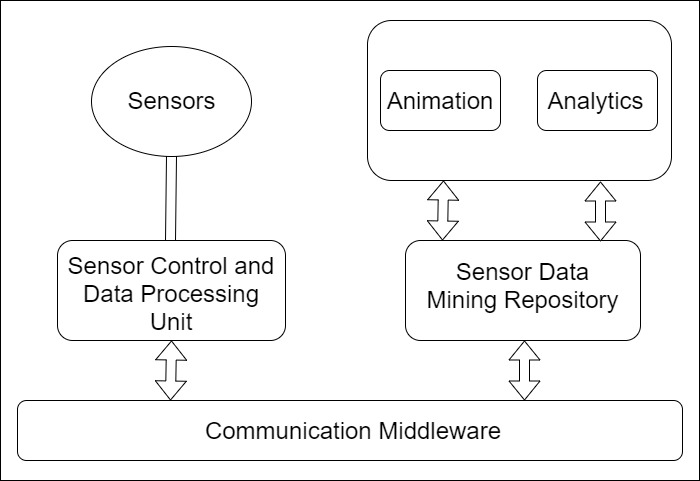
\includegraphics[scale=0.70]{images/figure2.png}
      \end{center}
      \caption{System Architecture}
      \label{mesh}
  
    \end{figure}


     \subsection*{Hardware Architecture}
\subsubsection*{Sensor Control and Data Processing Unit}
This unit is the core for the pollution monitoring as it is where all the other modules are connected including the communication middleware. This module does the following function:


\begin{enumerate}

\item Control the sensors in collecting data.
\item It filters and processes the collected data and forward to the software.
\item Provide the necessary voltage for all the hardware connected to it.

\end{enumerate}
For simplicity and ease of programming we have selected one of the most popular processor in market, Arduino Ethernet board which has ATmega328 microcontroller as shown in Fig.\ref{Arduino}. 

\begin{figure}[h]
  \begin{center}
  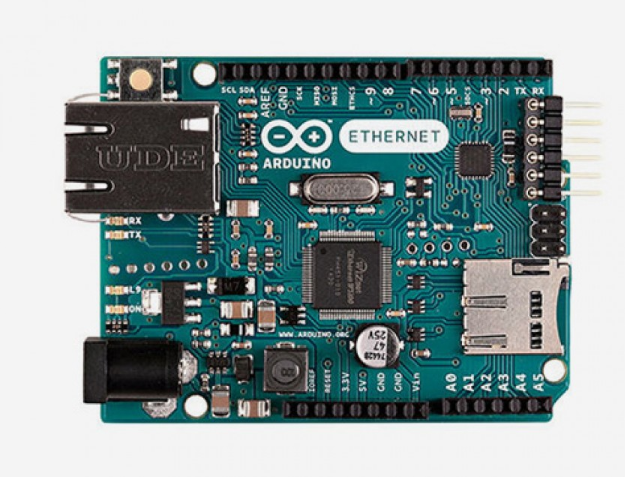
\includegraphics[scale=0.80]{images/figure3.png}
  \end{center}
  \caption{Arduino Ethernet Board}
  \label{Arduino}
\end{figure}

Arduino is an open source physical computing platform that is divided into two parts, one is the hardware which is the board itself in which the external components are added to and other is the software which is the development environment for the  processing language. It is very easy and simple to use the board with any external devices such as sensors or actuators and is widely used by researchers. There are different features which makes arduino popular and can be listed as \cite{Banzi2008}:


\begin{enumerate}


  \item Arduino is multi-platform and can be used with windows,mac and linux.

  \item The programming is done via USB cable and not serial port and is useful as modern computers don't have serial port.

  \item As it is open source hardware and software all the necessity for an external hardware to be worked on like circuit diagram, the code can be easily downloaded.
  
  \item There is an Integrated Development Environment (IDE) which can be used as an interface for talking with the hardware and is very simple.
  
  \item There is an active arduino forum in which many researchers or developers who are working on projects contribute their ideas and will help in trouble shooting.
  
  \item The cost of the hardware is very cheap and will come under 60 CAD and is easily affordable.
  
\end{enumerate}

The board can be powered either by using a FTDI cable/USB serial connector, external power supply or using an optical Power Over ethernet module (PoE). The ATmega328 has 2 KB of SRAM and 1 KB of EEPROM. The detailed specification\cite{Guti2017} of the board is given below in the table.
 
\begin{table}[h]
  \caption{Technical specification}
  \begin{tabularx}{\columnwidth}{X|X}
      \hline
      Description                 & specification    \\
      \hline
      Microcontroller & ATmega328P \\
      Operating Voltage & 5V\\
      Input Voltage Plug (recommended) & 7-12V\\
      Input Voltage Plug (limits)       & 6-20V\\
      Input Voltage PoE (limits)        & 36-57V \\
      Digital I/O Pins    & 14 (of which 4 provide PWM output)     \\
      Analog Input Pins & 6\\
      Flash Memory & 32 KB (ATmega328P) of which 0.5 KB used by bootloader\\
      SRAM     & 2 KB (ATmega328P)\\
      EEPROM   & 1 KB (ATmega328P) \\
      Clock Speed  & 16 MHz\\
      \hline
  \end{tabularx}
  \label{table:Technical specification}
\end{table}
 
Having all these specification gives the freedom for researchers to explore with different electronic devices easily. The board is programmed with the help of arduino programming language which is very close to embedded C language and it is done on Arduino development environment. 

\subsection*{Sensor}

Sensor networks are new instruments useful to detect the conditions in remote places in the physical world in environmental monitoring applications such as pollution monitoring, transportation management, intrusion detection and many more \cite{Jung2011}. With the constant development in electronics industry, it is possible to collect data remotely and collected data can be transferred to the required platform at a short period of time.
There are different sensors available in market which can measure the pollutants and display the value, but the idea here is to select the one which is of low cost and also gives the most accurate values.
\par
Having said that there is a variety of options available for sensors based on the way it measures the pollutants. One such category is Metal Oxide Semiconductor (MOS) gas sensor also known as semiconductor gas sensor, which is used to detect the concentration of any hazardous gases in the atmosphere by changing its resistance. The most popular series available in market for this category is MQ-XX sensors which is popular for its wide detecting scope, long life, stability, high sensitivity, fast response and also simple drive circuit \cite{Data2012}.The sensing material is made up either from Aluminum Oxide ($ Al_{2}O_{3}$) or Tungsten trioxide ($WO3$)based ceramic and has a coating of Tin Oxide $ SnO_{2} $ that acts as the sensing material for the desired gas. The sensing element is heated through Platinum wires which is connected to leads made up of Nickel-Chromium, well known conductive alloy. The gas to be detected has a specific temperature at which it gets ionized and the task of the sensor is to work at that temperature. Once the gas gets ionized it gets absorbed by the sensing material which changes the resistance and inturn changes the voltage across the sensor and can be read by the microcontroller \cite{gassensor}. The voltage value along with reference voltage and other resistor's resistance is used to find the resistance of sensor. Once the resistance of the sensor is known then by using the sensitivity curve the concentration could be found out. 

Another popularly used  MOS sensor which we explored was MICS which are MEMS based whose mode of operation is similar to the above said sensor as both of them are metal oxide. Here, oxidizing gas or the pollutant gas add to the insulative oxygen species causing the resistance to increase \cite{SGXSensortech}.
 Other than MOS sensors, we also took a look at optical sensor which are spectroscopic devices which uses light scattering principle to find the concentration of pollutants. These sensors are known for its detecting capability of particulate matter of different sizes and is one of the recent development in the field of air quality monitoring. Highly responsive, reliable and long life are the main highlights of this sensor.
 \subsubsection*{Selected Sensor}

 After understanding the wide range of sensor options in the market the sensors were selected based on their performance, availability, ease of integration, and cost. The selected sensors were:
 \begin{enumerate}

  \item MQ-2 Sensor: This is a a semiconductor gas sensor which has an electrochemical sensor which detects multiple gases such as Carbon monoxide, LPG, methane, and other combustible steam. The sensor is connected in series with a variable resistor to form a voltage divider circuit and the variable resistor is used to change the sensitivity. The sensitivity curve for the sensor is shown for different types of gases.
\par
\begin{figure}[h]
  \begin{center}
  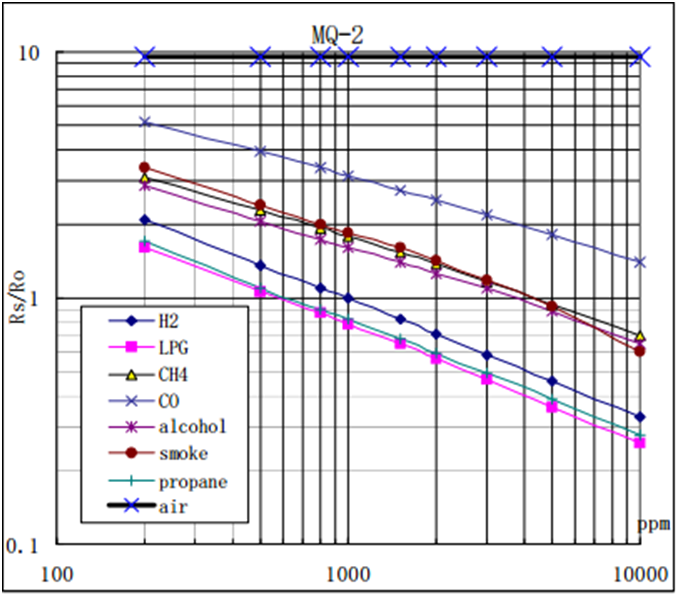
\includegraphics[scale=0.40]{images/figure1.png}
  \end{center}
  \caption{Sensitivity characteristics curve \cite{Data2012}}
  \label{curve}

  where $R_{o}$ is the sensor resistance in clean air and $R_{s}$ is the sensor resistance when exposed to gas.
\end{figure}
From the curve in Fig.\ref{curve}, the voltage across the sensor is found out depending on which gas one wants to detect and there after using this voltage value the concentration of pollutant is calculated. The range of detection of gas is from 100ppm to 10,000 ppm and has a high sensitivity and fast response time. The sensor is small and portable and provides integration in famous MCU platforms like arduino, raspberry pi etc. 

\item MQ 131: Another MQ-XX series sensor that we used for the system is for ozone. The working of the sensor is similar to MQ-2 sensor. It decreases the resistance when exposed to ozone and becomes more conductive when exposed to large concentration of the gas. This can be used to measure the concentration of ozone in air. The detecting concentration scope is from 10ppb to 2 ppm of ozone and also has a fast response time and long life.

\item MICS-2714: This is a robust MEMS sensor used for the detection of Nitrogen dioxide ($NO_2$). The detection range is from 0.05 to 10 ppm and has a response time of 10 seconds. The sensor is comparatively small and of low cost.

\item  PPD42NS Particulate sensor: The sensor detects the particulate matter through light scattering mechanism and consists of infrared LED positioned in forward angle to a photo diode. As soon as there is a variation in light density, the photo diode detects this and changes the current from the diode \cite{Allen2002}. The circuit generates a measurable signal known as Low Pulse Occupancy (LPO) which is proportional to PM concentration \cite{Kuula2017}. This sensor can measure both PM2.5 and PM10 concentration.

\item DHT11: This a very low cost sensor available in market for temperature and humidity measurement and has a calibrated digital output. The measurement range for temperature is from 0 degree to 50 degree Celsius. The device can be integrated to almost all platforms of Microcontroller and is considered to be the best choice for many applications.

 \end{enumerate}

 \subsection*{Communication Middleware}
 
 The collected data needs to be transferred to a platform so that user can understand and interpret the data from the sensor. We have used a WiFi module for this purpose, which will collect the data from the processor and transfers it to a IOT platform said to. The WiFi module used here is ESP8266, which is a highly integrated SOC that meets the requirement of user demand of efficient power usage, compact design and reliable performance\cite{Systems2018}. The ESP module can be connected to a processor or it can also be programmed on its own as the module itself is a MCU unit. Unlike the other sensor modules connected to the processor which needs a 5V power supply for its working, this module needs a 3.3V for its power up. The ESP module comes along with installed firmware from AI-thinker and it can be communicated with AT commands.On typing the AT command in the serial monitor the output would come as 'OK' if there is a successful connection. 

 This firmware can be replaced with user's own code which gives the power of flexibility of connecting with any IOT platform. The arduino platform supports the programming of ESP module which makes the integration much easier. The code can be written in the Arduino IDE and can be flashed into the ESP board by connecting it separately.
 The circuit for the ESP flashing is as shown which is a voltage divider circuit.[FIGURE NEEDS TO BE INSERTED] When the TX and RX pin of arduino is connected to TX and RX pin of the WiFi module it becomes in the programming mode and flashing occurs. 
 
 \section*{System Overview}
The complete circuit diagram of how the components are integrated to the Microcontroller is as shown is the figure \ref{system}. Each of these sensors were carefully arranged so that it reduces the spatial interferences. As majority of the sensors are heat sensors and discharges heat it affects the working of the sensor placed near to it. The initial arrangement of the sensors were done in the breadboard with wires. Building the circuit in breadboard gave the flexibility of working with different arrangements.

 \begin{figure}[h]
  \begin{center}
  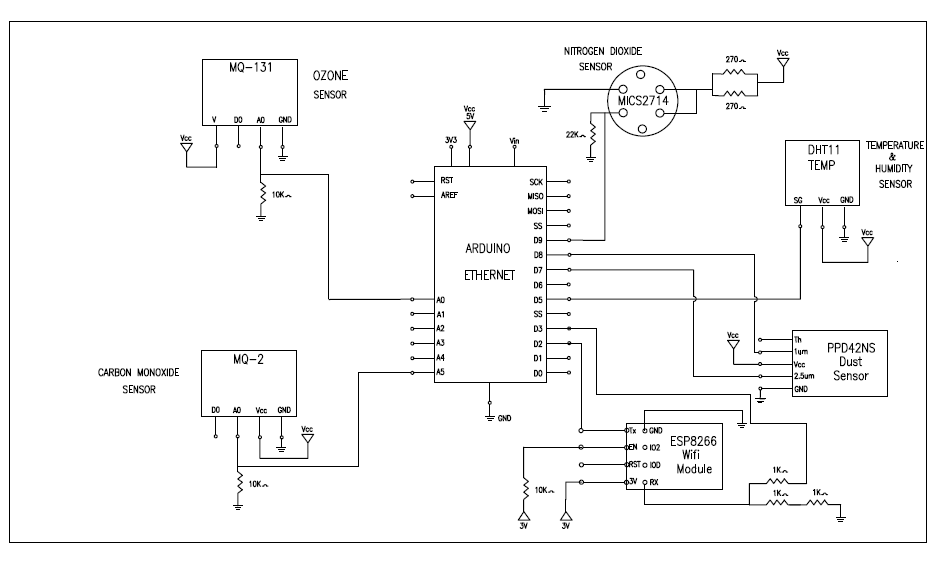
\includegraphics[scale=0.95]{images/figure5.png}
  \end{center}
  \caption{System Overview}
  \label{system}
\end{figure}

After building the circuit in breadboard, it was migrated to a Printed Circuit Board (PCB) developed by Flemings Solution Ltd, India. The design of the board is as shown in the figure \ref{pcb}. The PCB was designed in such a way that each sensors and the microcontroller itself was plug-in model to board. This was done so that in case of any malfunctioning of any of the sensors or processor, it could be replaced easily. The main advantage of using a PCB design is that all the components are fixed and there is no wiring at all. This produces a zero error circuit and there wont be any short circuiting.



\begin{figure}[h]
  \begin{center}
  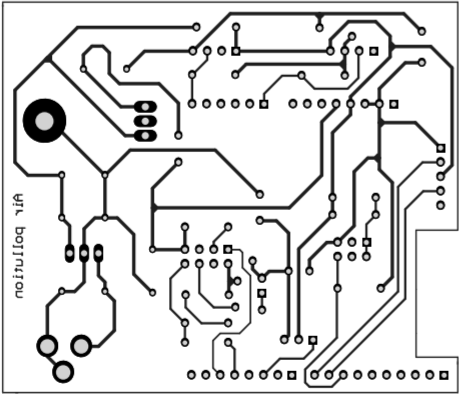
\includegraphics[scale=0.50]{images/figure10.png}
  \end{center}
  \caption{Printed Circuit Board}
  \label{pcb}
\end{figure}

\section*{IoT Architecture}

The hardware is the one responsible for the data collection but making these data available to user is done by the visualizing tool. The main objective which was kept when developing the system was the data collected should be accessed from anywhere and thats why IoT platforms were selected.

 \bibliographystyle{plain}
 \bibliography{chapter3}
 \end{document}
 
\documentclass[12pt,a4paper,oneside]{report}

\topmargin -.5in
\evensidemargin 0in
\oddsidemargin 0in
\textheight 9in
\textwidth 6.5in
\usepackage{url}
\usepackage{graphicx}
\usepackage{amsmath,amssymb,amsfonts}
\newtheorem{theorem}{Theorem}
\usepackage{float}
\usepackage{mathtools}
\usepackage{tabularx}

\begin{document}

\section*{Calibration Of Low Cost Sensor}

With the development of sensor technology for air pollution it has attracted a majority of researchers as well as common people to explore and understand more about the pollutants and its effects. This has given freedom for one to set up their own monitoring system at residences, office or even at schools. The problem with this is to identify how accurate the data collected from these commodity sensors to the reference monitoring system. If the system is giving values which is way too different from the reference value then it brings down the advantages of this technology. This issue can be dealt through calibration which will reduce the uncertainty in data and makes the output more accurate. 
\par 
Calibration can be defined as the act of evaluating and adjusting the precision and accuracy of measurement equipment \cite{Kejuruteraan2018}. If the measured output from the sensor is not equals to the actual output then it shows that there is a need for calibration. Usually all the electronic instruments are calibrated according to a particular conditions in the laboratory and acquires a certification of calibration before its sold out in the markets. Even then the measured value does not reach accuracy as the condition or the environment where it was calibrated changes that leaves the user with some raw values that gives no information. This issue was taken up and explored by a few researchers in the US Environmental Protection Agency(EPA) and came up with three so called 'Straw-Man Approach' to improve the usability of such data and presented in the Air sensor Workshop \cite{Williams2013}. 

The first approach was by a signal-based calibration technique which requires the data from the remote stations, which is the reference station, to be broadcasted to the local station where the sensor is located and will receive this data and performs a single point calibration of the response. This approach would have been easy if the sensor was already equipped with the data collection and would process automatic calibration. 

The next option for calibrating is called the direct sensor calibration that involves placing the sensor in a chamber in which a known concentration of pollutant is set and response is observed. As the concentration of the pollutant is already known the output curve can be compared with it and calibrated accordingly. This is the most common method used for calibration as is often called as laboratory evaluation. Another way of approaching direct calibration is by inspecting the pre-defined response given by the manufacturer and checking how accurate the sensor is to the given concentration. In either case the calibration requires equipment and skills to give accurate concentration value.

The last option is by secondary data normalization in which the concentration values of the pollutant from the low cost sensor is normalized in accordance with the federal reference method (FRM) or federal equivalent method (FEM) analyzers. This approach is cost effective when compared to the other techniques and easy to approach. This could be achieved by implementing machine learning algorithms that will convert the non-calibrated data into data of an acceptable form. 

\bibliographystyle{plain}
\bibliography{chapter4}
\end{document}
\chapter{Experimental Evaluations}




\chapter{Conclusion and Future work}



     %%%% Input file with Summary.tex
%\input{Chapter7}
%\input{Chapter8}


%%%%%%%%%%%%%%%%%%%%%%%%%% BIBLOGRAPHY %%%%%%%%%%%%%%%%%%%%%%%%%%%%%%%%%%%%
\clearpage
\addcontentsline{toc}{section}{Bibliography}  % Add to the content
\fancyhead{} % clear all header fields
\fancyfoot{} % clear all footer fields
\pagestyle{fancy}
\fancyhfoffset[L]{0 cm}
\rhead{\text{\thepage }{}}
\lhead{\textbf{Bibliography}}
\begingroup
%\setlength{\bibsep}{10pt}
\linespread{1}\selectfont
\bibliography{Thesis}     %%%% Input file with Thesis.bib
\endgroup

%%%%%%%%%%%%%%%%%%%%%%%% BIBLOGRAPHY %%%%%%%%%%%%%%%%%%%%%%%%%%%%%%%%%%%%

%%%%%%%%%%%%%%%%%%%%%%%%%% APPENDIX %%%%%%%%%%%%%%%%%%%%%%%%%%%%%%%%%%%%
%\clearpage
%\fancyhead{} % clear all header fields
%\fancyfoot{} % clear all footer fields
%\pagestyle{fancy}
%\fancyhfoffset[L]{0 cm}
%\rhead{\text{\thepage }{}}
%\lhead{\textbf{\appendixname\hspace{0.1cm} \thechapter{}}}
%\appendix
%\input{AppendixA}     %%%% Input file with AppendixA.tex
%\input{AppendixB}
%\input{AppendixC}
%\input{AppendixD


%%%%%%%%%%%%%%%%%%%%%%%%%%%%%%%%%%%%%%%%%%%%%%%%%%%%%%%%%%%%%%%%%%%%%%%%%%%%%
%\fancyhf{} % clear all header and footer fields
%\renewcommand{\chaptermark}[1]{\markboth{\chaptername\ \thechapter}{}}
%\renewcommand{\sectionmark}[1]{\markright{\thesection\ }}
%\fancyhf{}
%\fancyhead[RO]{\thepage}
%\fancyhead[LO]{\slshape\foottmark}
%\fancyhead[RE]{\slshape\leftmark}
%\addtocontents{toc}{\protect\contentsline{chapter} {Appendix}{}}
%\pagestyle{fancy} \fancyhfoffset[LE]{0 cm}
%\clearpage{\pagestyle{empty}\clearpage} \pagestyle{fancy}
%\renewcommand{\chaptermark}[1]{\markboth{\appendixname \ \thechapter}{}}
%\renewcommand{\sectionmark}[2]{\markright{\thesection\ #1}}
%\fancyhf{}
%\fancyhead[LE,RO]{\thepage} \fancyhead[LO]{\slshape\rightmark}
%\fancyhead[RE]{\slshape\leftmark}

%%%%%%%%%%%%%%%%%%%%%%%%%%%%%%%%%%%%%%%%%%%%%%%%%%%%%%%%%%%%%%%%%%%%%%%%%%%%%%%

\end{document}


